\documentclass{article}
% translate with >> pdflatex -shell-escape <file>

% This file is an extract of the PGFPLOTS manual, copyright by Christian Feuersaenger.
% 
% Feel free to use it as long as you cite the pgfplots manual properly.
%
% See
%   http://pgfplots.sourceforge.net/pgfplots.pdf
% for the complete manual.
%
% Any required input files (for <plot table> or <plot file> or the table package) can be downloaded
% at
% http://www.ctan.org/tex-archive/graphics/pgf/contrib/pgfplots/doc/latex/
% and
% http://www.ctan.org/tex-archive/graphics/pgf/contrib/pgfplots/doc/latex/plotdata/

\usepackage{pgfplots}
\pgfplotsset{compat=newest}

\pagestyle{empty}

\begin{document}
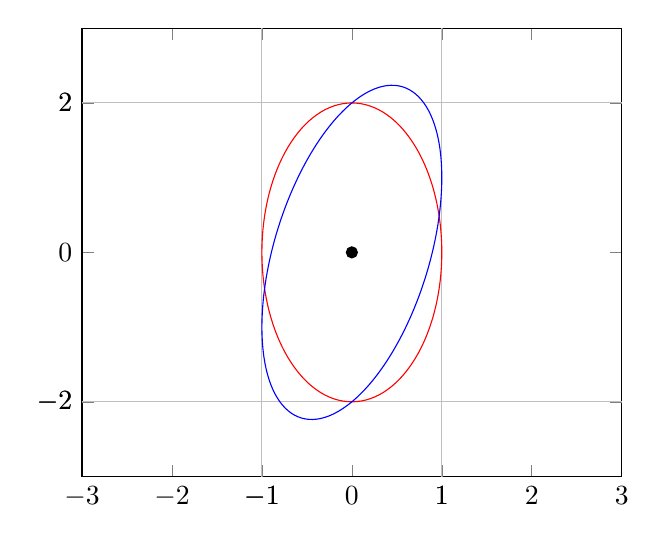
\begin{tikzpicture}
\begin{axis}[
	xmin=-3,   xmax=3,
	ymin=-3,   ymax=3,
	extra x ticks={-1,1},
	extra y ticks={-2,2},
	extra tick style={grid=major},
]
	\draw[red] \pgfextra{
	  \pgfpathellipse{\pgfplotspointaxisxy{0}{0}}
		{\pgfplotspointaxisdirectionxy{1}{0}}
		{\pgfplotspointaxisdirectionxy{0}{2}}
	  % see also the documentation of 
	  % 'axis direction cs' which
	  % allows a simpler way to draw this ellipse
	};
	\draw[blue] \pgfextra{
	  \pgfpathellipse{\pgfplotspointaxisxy{0}{0}}
		{\pgfplotspointaxisdirectionxy{1}{1}}
		{\pgfplotspointaxisdirectionxy{0}{2}}
	};
	\addplot [only marks,mark=*] coordinates { (0,0) };
\end{axis}
\end{tikzpicture}
\end{document}
